\section{Kompas w grze Skyrim}\label{chap:skrm}

The Elder Scrolls V: Skyrim (skrótowo Skyrim) jest to fabularna gra akcji o otwartym świecie, wyprodukowana przez Bethesda Game Studios i wydana przez Bethesda Softworks. Skyrim jest piątym tytułem z serii The Elder Scrolls oraz kontynuacją gry The Elder Scrolls IV: Oblivion. Jest to jednak nowa historią osadzoną w uniwersum The Elder Scrolls, a nie kontynuacją poprzednika. Fabuła opiera się na powrocie smoków do krainy Tamriel. Bohater okazuje się posiadać moc Głosu, dzięki czemu jest w stanie posługiwać się zaklęciami tych starożytnych stworzeń.
	Z punktu tworzonej przez nas gry, szczególnie interesujące jest  bardzo proste i sprytne rozwiązanie, jakim jest pasek przedstawiający pole widzenia gracza. Służy on między innymi jako kompas, ponieważ jedną z jego mechanik jest pokazanie użytkownikowi stron świata, znajdujących się w kierunku, w którym on patrzy. Pasek ułatwia także poruszanie się po świecie sygnalizując położenie wrogów, kompanów i ważnych dla rozgrywki lokalizacji.

    \begin{figure}[htbp]
        \centering
        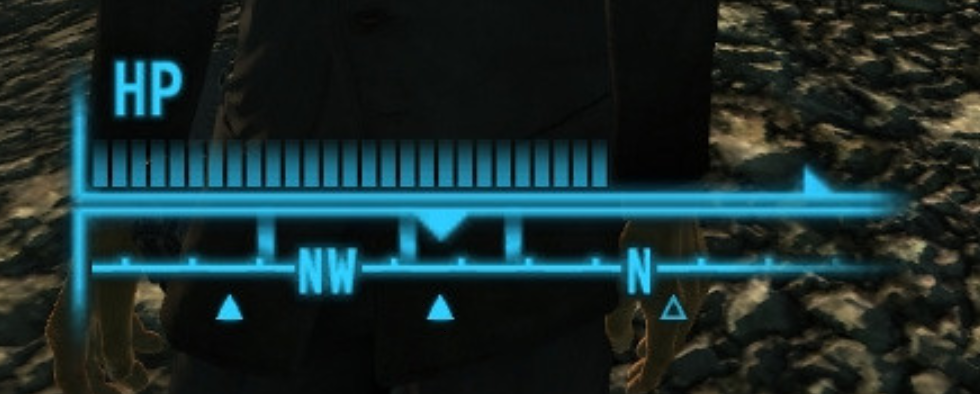
\includegraphics[width=0.9\textwidth]{images/ui/compassSkyrim.png}
        \caption{Pasek z gry The Elder Scrolls V: Skyrim ukazujący pole widzenia gracza. W tym momencie patrzy on delikatnie w prawo od południa (pokazuje to litera “S”). W jego zasięgu widzenia jest dwoje przeciwników (czerwone kropki) oraz jeden sojusznik (szara ikona po prawej).}\label{fig:Fallout}
    \end{figure}


